\chapter{Разработка метода программной редукции}
В соответствии с поставленной задачей, необходимо разработать метод редукции программ на языке Kotlin.
Разрабатываемый метод программной редукции является гибрибдным и состоит из следующих этапов: 
\begin{itemize}
	\item предварительное упрощение проекта;
	\item слайсинг;
	\item трансформации над СД;
	\item трансормации над текстовым представлением программы;
	\item иерархический дельта-дебаггинг;
\end{itemize}
Перечисленные этапы запускаются друг за другом в цикле до того момента, как тестовый пример не перестанет изменяться. Для каждого этапа программной редукции в данном разделе описан алгоритм работы и обоснована его актуальность.


\section{Проверка воспроизведения ошибки}
Изначально необходимо решить проблему проверки воспроизведения ошибки. Проблема состоит в том, что часто сообщения об одной и той же ошибке могут достаточно сильно различаться. Например, сообщение об ошибке компилятора может содержать часть сгенерированного байт-кода, и, при редукции, что логично, изменяться. 

Существует 2 способа решения данной проблемы. Первый --- при известном формате сообщения об ошибке производить его анализ и выделение необходимой информации. Данный способ хорошо применим к компиляторным тестам, где сообщение об ошибке имеет определенный формат. Пример такого сообщения приведен на рисунке~\ref{ex:error}. Как видно из рисунка, из сообщения можно выделить тип ошибки и ее местоположение.
\begin{figure}
\begin{lstlisting}
Error:Kotlin: [Internal Error] org.jetbrains.kotlin.codegen.CompilationException: Back-end (JVM) Internal error: wrong code generated
org.jetbrains.kotlin.codegen.CompilationException Back-end (JVM) Internal error: Couldn't transform method node:
test ()V:
   L0
    LINENUMBER 2 L0
   L1
    POP
   L2
...
Cause: AFTER mandatory stack transformations: incorrect bytecode
Element is unknownThe root cause was thrown at: MethodVerifier.kt:28
File being compiled at position: (1,1) in /home/stepanov/Kotlin/DynProj/src/Main.kt
...
\end{lstlisting}
\caption{\label{ex:error}Пример сообщения об ошибке для компилятора языка Kotlin}
\end{figure} 

Второй способ --- сравнивать непосредственно сообщения об ошибке. Для решения этой задачи подходит разностный алгоритм, предложенный В. Майерсом~\cite{myers1986ano}. Данный алгоритм принимает два файла и генерирует инструкции для превращения одного файла в другой. Инструкции могут быть двух типов: удаление из первого файла и вставка во второй. Количество таких конструкций должно быть минимально возможным. Данная задача эквивалентна задаче поиска наибольшей общей подпоследовательности (НОП). Для нахождения НОП удобнее всего построить граф редактирования. Пусть первый файл $A = a_1...a_N$ и второй файл $B = b_1...b_M$ --- последовательности длиной $N$ и $M$ соотстественно. Граф редактирования для $A$ и $B$ имеет узел в каждой точке в решетке $(x, y)$, где $x \in [0, N]$, и $у \in [0, M]$. Узлы графа соединены горизонтальными, вертикальными и диагональными направленными ребрами. Горизонтальные ребра соединяют каждый узел с правым соседом, вертикальные --- с соседом снизу. Если $a_x = b_y$, то тогда строится диагональное ребро соединяющее узлы $(x-1, y-1)$ и $(x, y)$. После построения графа задача сводится к поиску пути с наибольшим количеством диагональных ребер.
В рисунке~\ref{ex:lcs} приведен пример графа редактирования и такого пути для последовательностей A = abcabba и B = cbabac из статьи~\cite{myers1986ano}.
\begin{figure}	
		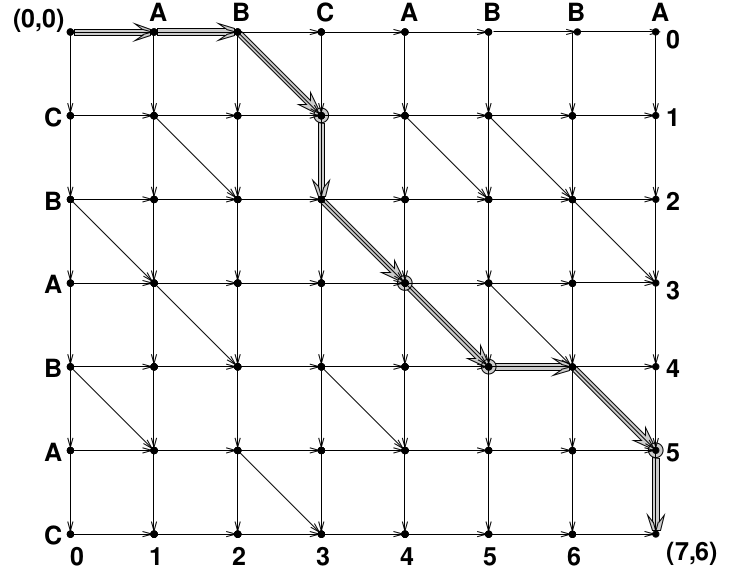
\includegraphics[width=0.99\linewidth]{fig/lcsexample} 
		\caption{\label{ex:lcs}Пример графа редактирования}
\end{figure}

\section{Предварительное упрощение проектов}
Современные программы имеют множество сложных внутренних связей, поэтому зачастую удаление нерелевантной к ошибке информации из целевого файла становится невозможным, поскольку данную информацию используют в другой части проекта. Для решения данной проблемы выполняется предварительное упрощение проекта --- упрощение файлов, импортирующих целевой файл с ошибкой. Для формирования выборки файлов для упрощения используются списки импортирований. Каждая позиция в таком списке содержит все конструкции, которые могут быть использованы из другого файла или пакета. 

В списке импортирований для языка программирования Kotlin может использоваться "*" --- знак обобщения импортирования. Это означает то, что из указанного пакета или файла импортируются все возможные конструкции. В разработанном алгоритме "*" заменяются на все возможные импортирования из указанного файла или пакета. Например, если в файле A содержатся классы \texttt{class1} и \texttt{class2}, а в классе B содержится импортирование \texttt{import A.*}, то он будет преобразован в \texttt{import A.class1} и \texttt{import A.class2}. 


Разработанный алгоритм сначала получает список всех конструкций, которые могут быть включены из целевого файла с ошибкой, затем рекурсивно проходит по всем файлам и строит дерево зависимостей, в котором каждый узел --- файл, а его глубина --- порядок его зависимости от целевого файла. После построения дерева, последовательно, начиная с наибольшей глубины, производится запуск упрощающих трансформаций над каждым узлом в дереве. Ниже приведен список трасформаций, каждая из которых подробно описана далее в этом разделе:
\begin{itemize}
	\item упрощение функций и свойств;
	\item набор трансформаций над текстовым представлением;
	\item удаление пустых управляющих конструкций;
	\item удаление неиспользуемых импортирований.
\end{itemize}

TODO переписать
TODO ввести синтасическое дерево (СД)
\section{Программный срез}
Алгоритмы слайсинга были подробно описаны в главе 1. Ввиду простоты реализации и популярности, был выбран статический слайсинг, который проводился над СД. Дальнейшие эксперименты показали, что данный вид программного среза в совокупности с другими методами редукции является достаточным по скорости и качеству работы. Стоит отметить, что главной проблемой слайсинга является обязательность наличия точной локации причины ошибки.
Программный срез производится на следующих уровнях:
\begin{itemize}
	\item классов;
	\item функций;
	\item внутрипроцедурном;
\end{itemize}
\subsection{Слайсинг на уровне классов и функций}
Слайсинг на уровне функция работает следующим образом. Из целевой функции производится рекурсивный обход всех вызовов из неё других функий и строится дерево использования, в котором корень --- функция с ошибкой. Далее функции, не входящие в построенное дерево удаляются из файла. Пример слайсинга на уровне функций представлен на рисунке~\ref{funslicing}
\begin{figure}
	\begin{lstlisting}
		fun funWithBug() {
			fun1()
		}
		
		fun fun1(){
			fun2()		
		}
		
		fun fun2(){}
		fun fun3(){}
	\end{lstlisting}
	Результат слайсинга:
	\begin{lstlisting}
		fun funWithBug() {
			fun1()
		}
		
		fun fun1(){
			fun2()		
		}
		
		fun fun2(){}
	\end{lstlisting}
	\caption{\label{funslicing}Пример слайсинга на уровне функций}
\end{figure}
\subsection{Внутрипроцедурный слайсинг}
Слайсинг производится при классическом, обратном обходе PSI, в один проход. Алгоритм принимает на вход строку, в которой содержится ошибка. Алгоритм внутрипроцедурного слайсинга приведен на рисунке~\ref{alg:interproceduralslicing}
\begin{figure}
\begin{algorithmic}[1]
\STATE $curLine \Leftarrow lastLine$
\WHILE{$curLine != line$} 
	\STATE $deleteLine(curLine)$
	\STATE $curLine \Leftarrow curLine - 1$
\ENDWHILE
\STATE $monitoringElems \Leftarrow parseLine(line)$
\STATE $curLine \Leftarrow curLine - 1$
\WHILE{$curLine != firstLine$} 
	\IF{$dependingOnError(curLine, monitoringElems)$} 
		\STATE $monitoringElems \Leftarrow monitoringElems + getVariables(curLine)$ 
	\ELSE 
		\STATE $deleteLine(curLine)$ 
	\ENDIF
\ENDWHILE
\end{algorithmic}
\caption{\label{alg:interproceduralslicing}Алгоритм внутрипроцедурного слайсинга}
\end{figure}


До момента попадания в строку, приводящую к программному сбою, производится удаление всех выражений. Далее производится разбор строки, содержащей ошибку и выделение всех содержащихся в ней переменных. После этого производится дальнейший проход по функции с проверкой влияния переменных, содержащихся в новой строке на переменные, влияющие на ошибку. Если найденные переменные влияют на ошибку, то они также начинают считаться переменными, влияющими на ошибку. Пример работы слайсинга приведен в главе 1.



\section{Трансформации над СД}
Опытным путем был образован необходимый набор трансформаций над СД. Дерево разбора в качестве редактируемого представления программы было выбрано ввиду сложности проведения данного типа трансформаций над текстовым представлением, а информации, которая в нем содержится, хватает для проведения запланированных трансформаций. Ниже приведено описание каждой трансформации. 

\textbf{Удаление комментариев}. Часто программа содержит большое количество комментариев, которые, очевидно, являются нерелевантной информацией по отношению к программной ошибке. Поэтому производится их удаление.

\textbf{Упрощение Элвис-оператора}. Система типов в языке программирования Kotlin нацелена на предотвращение ошибок, при которых происходит обращение к null значению. Поэтому система типов Kotlin отличает типы, которые могут иметь значение null(nullable), и которые не могут non-null). Если у нас есть nullable ссылка, благодаря элвис-оператору мы можем провести проверку этой ссылки на null и использовать ее в левой части оператора, либо использовать non-null значение в правой части оператора. И, если данный оператор не влияет на воспроизведение ошибки в программе, мы можем заменить его на правую часть. Например, выражение \texttt{val a = nullable ?: 42}, где \texttt{nullable} --- nullable ссылка, можно заменить на \texttt{val a = 42}.

\textbf{Удаление пустых управляющих инструкций}. Если какая-нибудь управляющая инструкция, например: if, for, try, when и т.д. не содержит тела и не влияет на воспроизведение ошибки, то можно ее удалить.

\textbf{Удаление наследования}. При редукции программы, использующей ООП, часто представляется невозможным удалить информацию, нерелевантную к ошибке из-за каких-либо внутренних связей(наследование и т.д.). Но в некоторых случаях это наследование можно попытаться упростить. Данная трансформация рекурсивно проходит по всем классам-родителям класса, в котором содержится ошибка и удаляет поля с одинаковыми именами. TODO: плохо описал, пример
\begin{lstlisting}
interface A {
    fun f()
}

open class B : A {
    override fun f() {}
}

class ClassWithBug : B() {
    override fun f() {}
    fun a() {}
}
\end{lstlisting}
\begin{lstlisting}
interface A {

}

open class B : A {

}

class ClassWithBug : B() {

    fun a() {}
}
\end{lstlisting}

\textbf{Удаление параметра из функции}. В результате применения различных методов редукции аргументы функции часто становятся неиспользуемыми. Для их удаления необходимо найти все вызовы данной функции и одновременно удалить параметр из функции и из всех ее вызовов. Необходимо учитывать, что в программе могут иметься другие функции с таким же названием и даже сигнатурой.

\textbf{Удаление значений из списка родительских классов}. В списке родительских классов, каждый класс, если он не влияет на возникновение программной ошибки, можно попытаться удалить, одновременно с этим необходимо удалить все перегружаемые члены из удаляемого класса.

\begin{lstlisting}
open class B {
    open val a = 1
    open val b = 2
    open fun f() {}
}

class ClassWithBug : B() {
    override val a = 2
    override val b = 1
    override fun f() {}
}
\end{lstlisting}

\begin{lstlisting}
open class B {
    open val a = 1
    open val b = 2
    open fun f() {}
}

class ClassWithBug {
    val a = 2
    val b = 1
    fun f() {}
}
\end{lstlisting}

\textbf{Удаление неиспользуемых импортирований и переводов строк}. При редукции часто многие импортирования становятся неиспользуемыми. Их логично удалять. Также при редукции могут оставаться лишние переводы строк, усложняющие читаемость результирующего кода, которые также удаляются.

\textbf{Замена возвращаемого значения функции на константу}. Если функция имеет стандартный возвращаемый тип, например Int или String, то правую часть оператора перехода return можно заменить на константное значение в случае, если замена не будет влиять на воспроизведение ошибки. Например, если функция имеет возвращаемый тип Int, то можно заменить правую часть всех операторов return на 0.

\textbf{Замена типа возвращаемого значения функции на Unit}. Функция, не возвращающая никакого значения, в языке программирования Kotlin имеет тип Unit (аналог void в Java). Стоит отметить, что тип возвращаемого значения Unit может быть опущен. По аналогии с предыдущей трансформацией, если она не влияет на воспроизводимость ошибки, можно заменить тип возвращаемого значения на Unit и удалить все операторы перехода return.

\textbf{Упрощение конструктора класса}. В результате редукции часто параметры из конструктора класса становятся неиспользуемыми. В этом случае их можно удалить. Для этого необходимо удалить неиспользуемый оператор непосредственно из конструктора и из всех его вызовов.

\textbf{Упрощение цикла for}. Часто для воспроизведения ошибки цикл for становится нерелевантным, а тело цикла используется. В документации языка программирования Kotlin описано, что цикл for позволяет проходить по всем элементам объекта, имеющего итератор:
обладающего внутренней или внешней функцией iterator(), возвращаемый тип которой обладает внутренней или внешней функцией next(), и обладает внутренней или внешней функцией hasNext(), возвращающей Boolean. Поэтому в случае использования параметра цикла необходимо создать свойство, левая часть которого будет этим параметров, а правая --- вызов функций iterator() и next() у объекта, по которому производится итерация. Например для цикла {\ttfamily for (item in collection)} необходимо создать свойство {\ttfamily val item = collection.iterator().next()} и далее подставить его тело.

\textbf{Упрощение функций и свойств}. В случае не влияния на воспроизведение ошибки, все тела всех функций и правую часть всех свойств можно заменить на вызов специальной функции TODO() --- при обращении бросающей исключение UnsupportedOperationException.

\textbf{Упрощение оператора if}. Данная трансформация заменяет оператор if на какую-либо его ветку, в случае успеха после теста на воспроизведение ошибки. Необходимо различать в условии оператора сравнение переменной с каким-либо значением, например if (i == 0) и сравнение с каким-либо типом при помощи оператора is, например if (item is Type). Во втором случае возможно появление умных приведений, так как компилятор следит за is-проверками для неизменяемых значений и вставляет приведения автоматически, там, где они нужны. Поэтому необходимо вручную приводить переменную из условия к типу, с которым он сравнивается для true-ветки. Для этого необходимо использовать оператор as: item as Type.

\textbf{Упрощение наследования}. Данная трансформация направлена на упрощение наследования. TODO подробнее!

\textbf{Упрощение лямбда-выражений}. Иногда в процессе редукции возникает возможность заменить лямбда-выражение на его тело, что и делает данная трансформация. 

\textbf{Упрощение оператора when}. Оператор when, в случае не влияния на воспроизведение ошибки, может быть заменен на выражение в else ветке. Также необходимо обращать внимание на возможную вложенность операторов и начинать с оператора с наибольшей вложенностью.
\begin{lstlisting}
fun main() {
    var a = 1
    when (a) {
        1 -> a++
        else -> a--
    }
}
\end{lstlisting}
\begin{lstlisting}
fun main() {
    var a = 1
    a--
}
\end{lstlisting}
\textbf{Упрощение блоков try-catch}. Содержимое данных блоков можно, в случае успешного воспроизведения ошибки, поменять на тело блока try.


\section{Трансформации над текстовым представлением программы}
Трансформации над текстовым представлением программы появились из-за того, что некоторые трансформации ввиду сложности и скорости нецелесооборазно производить над синтаксическим деревом. Примером такой трансформации может быть удаление какой-либо части текста, изменение подходящей под шаблон конструкции и т.д.

Первая трансформация из набора --- удаление текста внутри сбалансированной пары скобок. Скобки в языке программирования kotlin могут быть 4-х видов: фигурные, круглые, квадратные и треугольные. Данная трансформация находит все сбалансированные скобки в программе и пытается удалить весь текст внутри. В случае успешного воспроизведения ошибки с новым текстом программы данная трансормация применяется, в противном случае --- все возвращается обратно и производится переход к другой паре сбалансированных скобок. Следующая трансформация --- удаление скобок, поскольку часто в результате редукции появляются лишние скобки. Также в качестве дополнительной трансформации была придумана трансформация, удаляющая текст между каждой пары точек. Таким образом может быть удален лишний вызов функции. Например item.fun1.fun2 преобразуется в item.fun2

Следующий набор трансформаций --- замена текста, подходящего под шаблон. Данные трансформации могут быть трех видов:
\begin{itemize}
	\item замена текста, подходящего под шаблон, например "1294" на "0"; 
	\item замена части текста, подходящего под шаблон, на другой, например "i = i + 1" на "i++";
	\item применить к тексту, подходящему под шаблон другой шаблон, например "a + b + c + d" на "a + b".
\end{itemize}
Ниже приведен список разработанных шаблонов и их замен:
\begin{itemize}
	\item замена арифметических операторов += на =;
	\item замена while на if;
	\item замена всех целочисленных констант на 0 и 1;
	\item замена строковых констант на "";
	\item замена всех типов на целочисленный;
	\item упрощение бинарных операций.
\end{itemize}
\begin{lstlisting}
fun f() {
    var a = 124125125
    val b = a + 1
    val c = 1.1
    var d: Double
    while (a.toDouble() != c) {
        d = a * b * c
        a += 1
    }
}
\end{lstlisting}

\begin{lstlisting}
fun f() {
    var a = 0
    val b = a + 1
    val c = 0.0
    var d: Double
    if (a.toDouble() != c) {
        d = a
        a++
    }
}
\end{lstlisting}


\section{Иерархический дельта-дебаггинг}
Иерархический дельта-дебаггинг является заключительной трансформацией и удаляет ту нерелевантную информацию, которую оставили предыдущие трансформации. Алгоритмы дельта-дебаггинга и иерархического дельта-дебаггинга приведены в главе 1. Алгоритм работает с синтаксическим деревом. Поочередно к каждому уровню дерева, начиная с верхнего, применяется алгоритм классического дельта-дебаггинга, который находит минимальную конфигурацию на данном уровне и удаляет из дерева нерелевантные узлы. Данная трансформация может порождать синтаксически неверный код, что необходимо обрабатывать, так как проверка синтаксической корректности происходит намного быстрее, чем запуск теста и обработка сообщения об ошибке.